\chapter{The Flaws of the Similarity Assumption}\label{chap:flaws}
% ---- TAKEAWAYS ----
% - General-purpose representations are built for all of chemistry. On one dataset, most of their features barely vary.
% - Some representations give different molecules exactly the same vector, mostly stereoisomers. No model can tell those molecules apart.
% - A similarity or distance compares every feature, so features irrelevant to the task dilute it. Different representations also disagree about which molecules are close.
% - Methods that judge a molecule by its neighbors did worst under label noise: LNL methods that use a distance, and noise detection by neighbors.
% - What is needed is a compact set of features chosen for the task from several representations. Chapter 5 builds it: the hybrid.
% ---- END TAKEAWAYS ----
% ---- NOTES: The Flaws of the Similarity Assumption ----
% Takeaway: before the first section, say that one section reuses the confirmation report's LNL study.
% Paragraph 1: a short preamble, opening with \textit{Preamble.} as in Chapter~\ref{chap:robustness}.
% - Section \ref{sec:lnl_motivation} reuses the exploratory learning-with-noisy-labels study from the DPhil confirmation report.
% - The report is titled "Investigating the Effects of Noise on Molecular Property Prediction". It is unpublished (January 2026).
% - The text and numbers of that section are identical or similar to the report. The rest of the chapter is new.
% - Cite it once here as \citet{Punt2026confirmation}.
% - refs.bib entry needed: @unpublished{Punt2026confirmation, author = {Punt, Adelaide}, title = {Investigating the Effects of Noise on Molecular Property Prediction}, note = {DPhil confirmation report, University of Oxford}, year = {2026}}.
% ---- END NOTES ----

% [TRIM3 2026-09-30] simplified
% CODE INPUT
% [TRIM2 2026-09-30] numbers removed, same points in words
% TODO: review, needs manual review
% [RESTORE 2026-09-30] Ch4-1
This chapter asks whether the standard ways of comparing molecules suit the dataset and task at hand. Because general-purpose representations are built for all of chemistry, we first count how many of their features vary on a single dataset. On hERG $K_i$, most ECFP4 features take a single value in almost every molecule. In an exploratory study of learning with noisy labels, the configurations with the lowest retention under noise all used a distance, and noise detection by neighbors usually made the model worse.



\section{Introduction}
% [notes moved to thesis_notes_moved.md]

% [TRIM2 2026-09-30] typos fixed only
% TODO: review, needs manual review
One of the fundamental assumptions in cheminformatics, the similar property principle (Chapter~\ref{chap:background}), is that two structurally similar compounds display similar chemical properties \citep{Johnson1990}; we call it the similarity assumption. While there are important exceptions, namely activity cliffs \citep{Stumpfe2012, vanTilborg2022}, this is a well-established concept. However, there is no single way to define similarity between compounds, and this is where the assumption begins to break down in practice. When defining similarity between two molecules, we typically rely on some pairwise mathematical function, or coefficient, that takes in two molecular representations as input. Two factors vary here, the representation and the coefficient. \citet{Bajusz2015} found that among standard coefficients, the choice between them matters little. This chapter questions the underlying representation. 

General-purpose molecular representations are designed to work across chemical domains. Consequently, when considering data from a specific domain, many of their features show little to no variance. Some representations assign separate molecules identical feature vectors. Since common fingerprints do not encode stereochemistry \citep{orsi2024map4c}, they are often unable to differentiate stereoisomers, which can have substantially different measured activity \citep{Nguyen2006}. As these coefficients compare every feature, irrelevant features dilute the result. Different representations also disagree about which molecules are close based on the information they carry. 


% [TRIM2 2026-09-30] typos fixed only
The problem of whether neighboring molecules can predict chemical activity has been measured before. The modelability index of \citet{Golbraikh2014} scores a binary dataset by the proportion of nearest-neighbor pairs that share an activity class, producing a single value for how strongly the similarity assumption holds on that particular combination of representation and data. It is not clear whether a low value is due to the data being intrinsically hard to model or to the representation not capturing adequate features for the task. Other work in this area relates to activity cliffs. \citet{Sheridan2020} compared experimental error, activity distribution and activity-cliff metrics as predictors of how well a dataset can be modeled, and found the cliff metrics the strongest of the three. However, they found that these metrics cannot separate real cliffs from  those produced by uncertain activity measurements. \citet{MedinaFranco2013} point out that some of these activity cliffs are artifacts of the chosen representation, similarity threshold, or noise in the data. Activity cliffs are distinct from noise, as they carry some of the most valuable information about the interaction between structure and activity. None of these measures ask specifically about whether the specific features within these representations matter for the property at hand. 


% [TRIM2 2026-09-30] typos fixed only
% TODO: review, needs manual review
There has been work that looks into how much the choice of representation changes the similarity measure. \citet{Riniker2013} benchmarked 12 fingerprints for similarity across 3 public datasets and found high correlations between them; only two simple baseline fingerprints differed significantly from the rest. The same was found for learned embeddings as neural embeddings gave negligible or no improvement over ECFP across 25 pretrained models and 25 datasets \citep{Praski2025}. \citet{Huber2026} did find a difference between the structure of the fingerprints. Measured using a graph-based structural reference, fingerprints that store raw counts improve agreement with the reference over folded fingerprints. The process of folding introduces bit collisions that distort similarity for molecules with many bits set \citep{Huber2026}. Activity cliffs follow the same pattern: across 15 combinations of representation and similarity measure on 3 datasets, the representations disagreed about which pairs form cliffs \citep{DabrowskiTumanski2026}. This supports the point \citet{MedinaFranco2013} make about cliffs as artifacts of their representation. Any method built on similarity, such as activity-cliff detection or editing a training set by its nearest neighbors \citep{Wilson1972}, inherits this choice, as do the noise estimation and mitigation methods of this thesis. \citet{Coupry2022} learn a molecular similarity from graph embeddings, but independently of any endpoint. \citet{Zheng2000} did choose the similarity for the task. They predict each molecule's activity as the average over its $k$ most similar molecules by Euclidean distance over descriptors, and choose the descriptors by simulated annealing to maximize the leave-one-out $q^2$. \citet{Itskowitz2005} also optimize the number of neighbors and their weighting. Both select features for a nearest-neighbor model of one endpoint, whereas this thesis selects features across several representations.

The purpose of this chapter is to establish the problem that Chapter~\ref{chap:method} sets out to solve. Section~\ref{sec:flaws:representations} asks, for a given dataset, how much the features of standard representations vary and how many molecules map to identical feature vectors. Section~\ref{sec:flaws:similarity} asks what happens when these features are used to quantify similarity, and Section~\ref{sec:flaws:consequences} follows the consequences for methods built on these similarity measures, including an exploratory study of LNL methods (Section~\ref{sec:lnl_motivation}).


\section{Flaws in Standard Base Representations}\label{sec:flaws:representations} % CODE INPUT: label added, needs review
% [notes moved to thesis_notes_moved.md]

% TODO: review, needs manual review
To quantify similarity between two compounds, we must first choose a representation to encode each compound. If the features within these representations are flawed, the similarity measure inherits them. Many standard representations are built to represent compounds across a wide array of chemical domains and be task-independent. However, chemical datasets often only cover a small region of the chemical space, leaving these general-purpose representations to describe chemistry which is absent from the dataset at hand. Some representations are easier to read chemically than others. Each PDV feature is a named physicochemical property, so its meaning is known, whereas the features of a frozen embedding, taken from the last layer of a network, do not say what chemical information, if any, they carry.

% TODO: come back to this


% CODE TODO [handled, see CODE INPUT blocks below]: Implement this and write it up. 
\subsection{Constant and Near-Constant Features}\label{sec:flaws:constant} % CODE INPUT: label added, needs review
% [TRIM3 2026-09-30] simplified
% [notes moved to thesis_notes_moved.md]
% ==== CODE INPUT: new, needs review ====
% Replaces the line: \todo[inline, color=yellow!40]{4.2.1: constant and near-constant feature counts (Table 4.1).}
% Numbers: scratchpad/thesis_code_todo/constant/constant_counts.json (scripts count_constant.py, mhg_dead.py, make_outputs.py in the same folder).
% Counts are on the saved feature matrices in rep_cache/<dataset>/<rep>.npy, all molecules of each dataset, no folds.
% [RESTORE 2026-09-30] Ch4-2
ECFP4 (Chapter~\ref{chap:background}) is built to describe any molecule before any dataset or task is known \citep{rogers2010}. A single dataset often comes from a few chemical series, so most bits are off in almost every molecule. The features that matter for a task form a small subset of those that vary, and which subset matters depends on the task. Here we count only how many features vary at all; Chapter~\ref{chap:method} asks which of them relate to the task.

% [TRIM3 2026-09-30] simplified
% TODO: molecule counts in this chapter differ from Chapter 3 with no reason given: hERG K_i 1,412 here against 1,415 in Chapter 3 (only the ties paragraph says 'deduplicated by InChIKey'), Caco-2 2,158 against 2,161, LogD 5,028 against 5,039, QM9 9,978 against 10,000 per replicate. The ChemBERTa-77M-MTR sentence in 'Molecules with identical feature vectors' uses 1,415. Add one sentence saying why once verified.
% TODO: the 384-feature ChemBERTa-77M-MTR embedding is called 'ChemBERTa' in Chapter 3 but 'ChemBERTa-2' in Table tab:constant_features (Chapter 2 uses both names). Pick one.
% TODO: review, needs manual review
A constant feature takes one value in every molecule of a dataset. A near-constant feature takes one value in at least 95\% of the molecules, so the near-constant count includes the constant features. We counted both, on all molecules, for the base representations (the representations the hybrid of Chapter~\ref{chap:method} selects features from, Table~\ref{tab:dataset_reps}) of hERG $K_i$, Caco-2, LogD, QM9, MDR1--MDCK efflux, human liver microsome (HLM) clearance, rat liver microsome (RLM) clearance and the Lhasa hERG blocker training set, and for the MACCS keys wherever they were computed. HLM clearance and the Lhasa hERG set are not in Table~\ref{tab:dataset_reps}; their base representations are those with counts in Table~\ref{tab:constant_features_b}.

% [TRIM3 2026-09-30] simplified
On these datasets the hashed substructure fingerprints have the most near-constant features, and the learned embeddings have none except MHG-GNN (Tables~\ref{tab:constant_features} and~\ref{tab:constant_features_b}, Figure~\ref{fig:constant_features}). ECFP4 on hERG $K_i$ (1,412 molecules; these datasets are curated as in Chapter~\ref{chap:method}, so their sizes differ slightly from Chapter~\ref{chap:robustness}, Additional file~\ref{app:datasets:ch3}) has 1,815 near-constant features out of 2,048. Across the seven datasets where ECFP4 is a base representation, this count runs from 1,815 to 1,997 (QM9, 9,978 molecules). The same 292 of MHG-GNN's 1,024 features are zero in every molecule on all seven datasets that use it, so they come from the saved encoder output rather than the data; we have not checked why. The Weisfeiler--Lehman (WL) graph kernel keeps only labels present in at least 5\% of a dataset's molecules, and on these datasets it has no near-constant features.

\begin{figure}[!htbp]
\centering
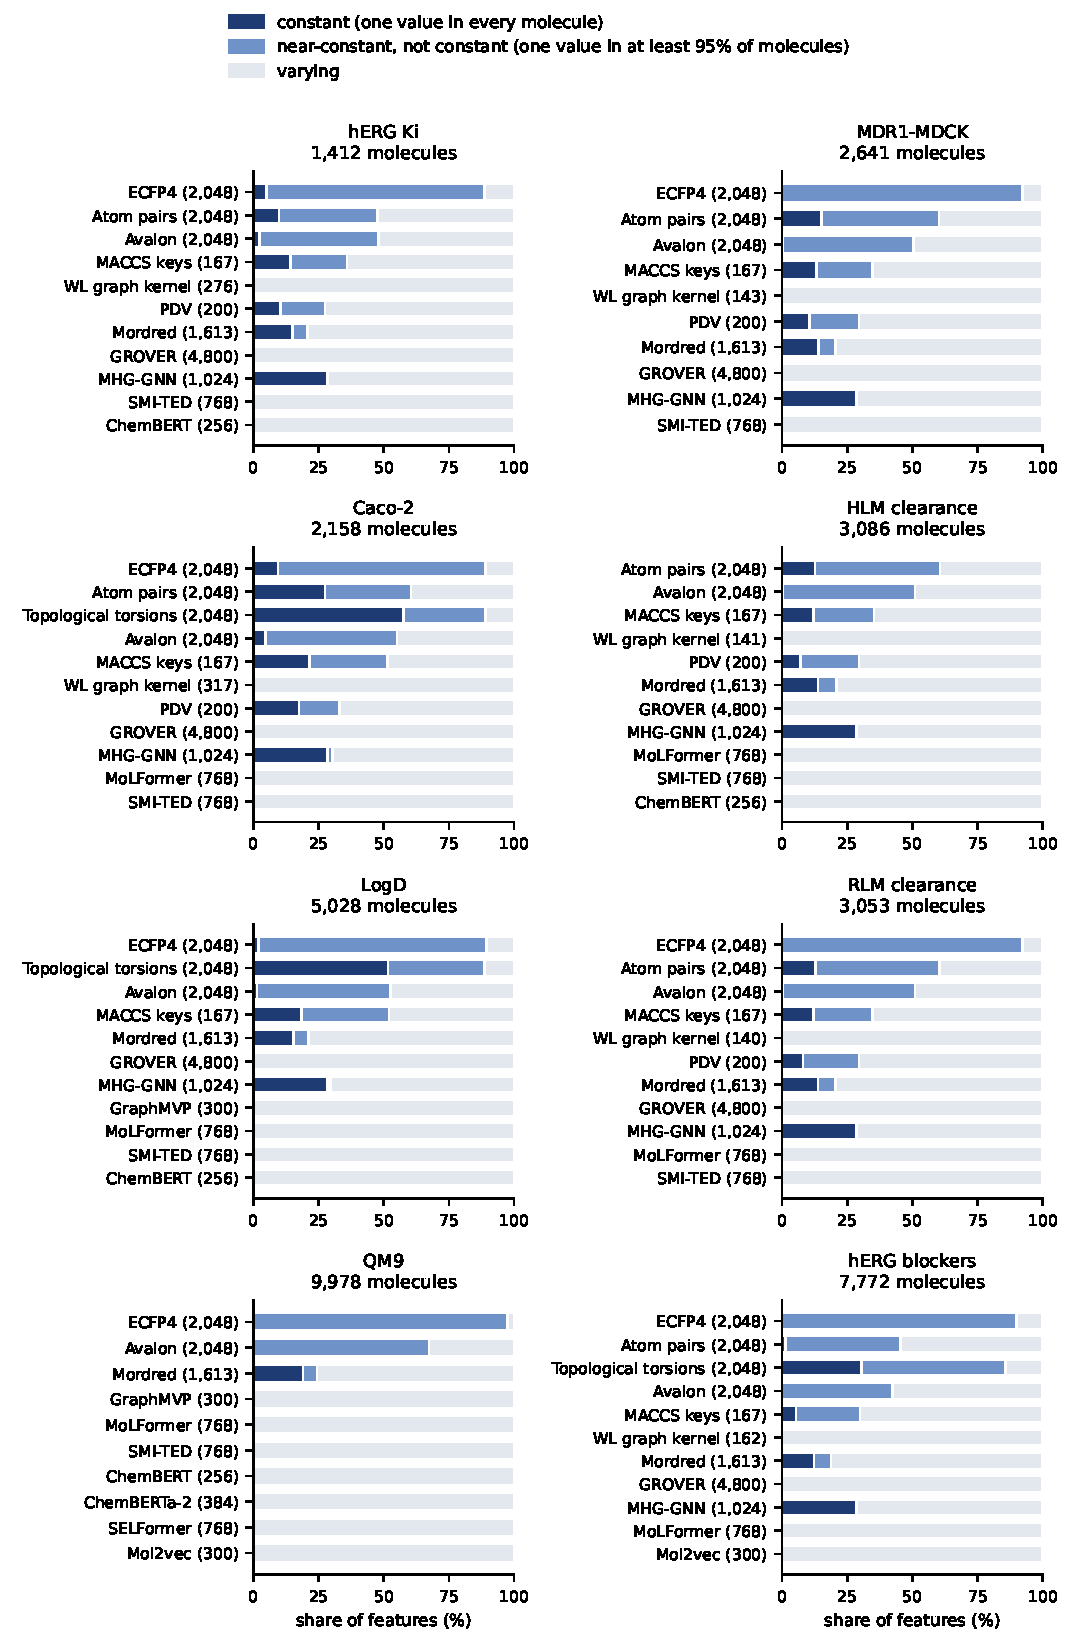
\includegraphics[width=\textwidth,height=0.72\textheight,keepaspectratio]{figures_code_input/constant_features.pdf}
\caption[Shares of constant, near-constant and varying features per representation.]{Shares of constant (dark blue), near-constant (mid blue) and varying (gray) features of each representation on eight datasets. The number of features of each representation is in parentheses.}
\label{fig:constant_features}
\end{figure}

% [TRIM3 2026-09-30] simplified
% [TRIM 2026-09-30] shortened
% TODO: review, needs manual review
Which count matters depends on the distance. Tanimoto similarity (Equation~\ref{eq:tanimoto}; the distance is $1-T$) ignores bits off in both molecules, but a bit on in every molecule raises every similarity slightly. All 105 constant ECFP4 bits on hERG $K_i$ are off. After standardization, a constant feature adds zero to a Euclidean or Manhattan distance, but a near-constant feature takes large values on the few molecules with the minority value. A bit on in 5\% of molecules becomes 4.36 on those molecules, and a bit on in one of the 1,412 hERG $K_i$ molecules becomes 37.56.

% [TRIM 2026-09-30] shortened
% [TRIM3 2026-09-30] paragraph removed

% [TRIM3 2026-09-30] paragraph removed

% [TRIM 2026-09-30] paragraph removed, text in cuts file

\todo[inline]{TODO: every cell of this table must hold a count. The dashes are representations outside that dataset's base representations; handoff in HANDOFF\_fill\_constant\_features\_tables.md.}
\begin{table}[htbp]
\centering
\small
\setlength{\tabcolsep}{4pt}
\begin{adjustbox}{max width=\textwidth,max totalheight=0.78\textheight}
\begin{tabular}{lrcccc}
\toprule
Representation & Features & hERG $K_i$ & Caco-2 & LogD & QM9 \\
 & & (1,412) & (2,158) & (5,028) & (9,978) \\
\midrule
ECFP4 & 2,048 & 105 / 1,815 & 194 / 1,826 & 39 / 1,834 & 0 / 1,997 \\
Atom pairs & 2,048 & 201 / 977 & 563 / 1,239 & -- & -- \\
Topological torsions & 2,048 & -- & 1,179 / 1,822 & 1,059 / 1,818 & -- \\
Avalon & 2,048 & 50 / 985 & 98 / 1,128 & 30 / 1,076 & 4 / 1,380 \\
MACCS keys & 167 & 24 / 60 & 36 / 86 & 31 / 87 & n/a \\
WL graph kernel & 140--317 & 0 / 0 / 276 & 0 / 0 / 317 & -- & -- \\
PDV & 200 & 21 / 55 & 35 / 66 & -- & -- \\
Mordred & 1,613 & 242 / 336 & -- & 247 / 340 & 307 / 394 \\
GROVER & 4,800 & 0 / 0 & 0 / 0 & 0 / 0 & -- \\
MHG-GNN & 1,024 & 292 / 292 & 292 / 310 & 292 / 304 & -- \\
GraphMVP & 300 & -- & -- & 0 / 0 & 0 / 0 \\
MoLFormer & 768 & -- & 0 / 0 & 0 / 0 & 0 / 0 \\
SMI-TED & 768 & 0 / 0 & 0 / 0 & 0 / 0 & 0 / 0 \\
ChemBERT & 256 & 0 / 0 & -- & 0 / 0 & 0 / 0 \\
ChemBERTa-2 & 384 & -- & -- & -- & 0 / 0 \\
SELFormer & 768 & -- & -- & -- & 0 / 0 \\
Mol2vec & 300 & -- & -- & -- & 0 / 0 \\
\bottomrule
\end{tabular}
\end{adjustbox}
\caption[Constant and near-constant features per representation, part 1.]{Constant and near-constant features of each representation on hERG $K_i$, Caco-2, LogD and QM9, with the number of molecules under each dataset name. Each entry gives the number of constant features and the number of near-constant features (one value in at least 95\% of molecules); WL graph kernel entries add its number of features, which varies by dataset. A dash marks a representation outside the dataset's base representations, and n/a one that was not computed.}
\label{tab:constant_features}
\end{table}

\todo[inline]{TODO: every cell of this table must hold a count. The dashes are representations outside that dataset's base representations; handoff in HANDOFF\_fill\_constant\_features\_tables.md.}
\begin{table}[htbp]
\centering
\small
\setlength{\tabcolsep}{4pt}
\begin{adjustbox}{max width=\textwidth,max totalheight=0.78\textheight}
\begin{tabular}{lrcccc}
\toprule
Representation & Features & MDR1--MDCK & HLM clearance & RLM clearance & hERG blockers \\
 & & (2,641) & (3,086) & (3,053) & (7,772) \\
\midrule
ECFP4 & 2,048 & 1 / 1,890 & -- & 1 / 1,887 & 0 / 1,840 \\
Atom pairs & 2,048 & 308 / 1,233 & 260 / 1,240 & 262 / 1,238 & 28 / 929 \\
Topological torsions & 2,048 & -- & -- & -- & 625 / 1,754 \\
Avalon & 2,048 & 5 / 1,032 & 8 / 1,044 & 8 / 1,045 & 0 / 866 \\
MACCS keys & 167 & 22 / 58 & 20 / 59 & 20 / 58 & 9 / 50 \\
WL graph kernel & 140--317 & 0 / 0 / 143 & 0 / 0 / 141 & 0 / 0 / 140 & 0 / 0 / 162 \\
PDV & 200 & 21 / 59 & 14 / 59 & 16 / 59 & -- \\
Mordred & 1,613 & 226 / 331 & 222 / 336 & 222 / 331 & 197 / 304 \\
GROVER & 4,800 & 0 / 0 & 0 / 0 & 0 / 0 & 0 / 0 \\
MHG-GNN & 1,024 & 292 / 292 & 292 / 293 & 292 / 293 & 292 / 292 \\
MoLFormer & 768 & -- & 0 / 0 & 0 / 0 & 0 / 0 \\
SMI-TED & 768 & 0 / 0 & 0 / 0 & 0 / 0 & -- \\
ChemBERT & 256 & -- & 0 / 0 & -- & -- \\
Mol2vec & 300 & -- & -- & -- & 0 / 0 \\
\bottomrule
\end{tabular}
\end{adjustbox}
\caption[Constant and near-constant features per representation, part 2.]{Constant and near-constant features of each representation on MDR1--MDCK efflux, HLM clearance, RLM clearance and the Lhasa hERG blocker training set of 7,772 molecules. Entries read as in Table~\ref{tab:constant_features}.}
\label{tab:constant_features_b}
\end{table}

% [TRIM3 2026-09-30] simplified
RDKit's MACCS keys include an unused bit 0, hence 167 features. All constant Mordred features are zero in every molecule, except one of the 307 on QM9, which is 1. Missing or infinite descriptor values are set to 0 (Chapter~\ref{chap:method}, ``Representations by domain''), so some may be descriptors that failed to compute; we have not checked which.

% Uni-Mol v2 is left out of both tables. Its saved features are zero in every molecule on hERG Ki, LogD, MDR1-MDCK, HLM, RLM and the Lhasa hERG set (6 datasets, 768 features each). It is not in any dataset's base representations.
% The Lhasa hERG set appears once: rep_cache/herg and rep_cache/lhasa_herg hold the same 7,772 SMILES in the same order with the same labels.

% ==== END CODE INPUT ====


\subsection{Molecules with Identical Feature Vectors}
% [notes moved to thesis_notes_moved.md]

A standard fingerprint- or descriptor-based representation can produce the same feature vector for two separate molecules. In turn, models using this representation will produce a single prediction for the molecules with identical features. Identical feature vectors do not always mean that the representation has merged two different molecules, since a dataset pooled from several sources can hold two measurements of the same molecule.


% [TRIM2 2026-09-30] SMI-TED hERG Ki tie count 52 -> 56 (ties_results.json: smited tied 56, stereo_only 56)
% [CH3 CHECK 2026-09-30] "explained in Chapter 2" changed to a plain pointer: Chapter 2 names the Weisfeiler--Lehman test but does not explain it.
% TODO: Chapter 2 says ECFPs are "typically" built with chirality flags on; this paragraph says ours are built with stereochemistry off. Consider saying so explicitly, and check which setting the Chapter 3 pipeline used.
% TODO: review, needs manual review
Many fingerprints are computed without stereochemistry \citep{orsi2024map4c}. In this research, ECFP4 is built with stereochemistry off, and the 2D descriptor sets (PDV, Mordred) also ignore it, so almost every molecule they tie is a stereoisomer of another (Table~\ref{tab:flaws:ties}). Any representation read from the 2D graph merges stereoisomers, since the two share an identical graph. Separately, methods using the Weisfeiler--Lehman relabeling scheme are bounded by the 1-Weisfeiler--Lehman test (Chapter~\ref{chap:background}), so some non-isomorphic graphs also receive the same vector; the graph-kernel features tie 105 of 1,412 hERG $K_i$ molecules, 56 of which differ only in stereochemistry and 49 in more than that. Whether a learned embedding differentiates stereoisomers is up to its individual implementation. SMI-TED, a pretrained SMILES encoder, ties 56 hERG $K_i$, 633 LogD and 177 Caco-2 molecules, all stereoisomers. A tokenizer can drop stereochemistry before the model even sees the input string. The tokenizer of the ChemBERTa-77M-MTR checkpoint (ChemBERTa-2 in Table~\ref{tab:constant_features}, called ChemBERTa in Chapter~\ref{chap:robustness}) gives 72 of the 1,415 hERG $K_i$ molecules of Chapter~\ref{chap:robustness} the same token sequence as another molecule. If stereoisomers did not differ in activity, this would not matter. However, stereoisomers can differ in measured activity \citep{Nguyen2006}, meaning these representations are all lacking potentially important chemical information.

% [TRIM3 2026-09-30] simplified
% CODE TODO [handled, see CODE INPUT blocks below]: paragraphs 4/5/6 + table + figure. Basically finish it out
% ==== CODE INPUT: new, needs review ====
% Numbers: scratchpad/thesis_code_todo/ties/ties_results.json (script ties/ties.py; table rows ties/table.py; figure ties/figure.py, pair in ties/figure_pair.json).
% Paragraph 4: the measurement.
For each dataset and representation, we grouped molecules with identical stored feature vectors. A tied molecule is a repeat if another molecule in its group has the same InChIKey, a featurization failure if its vector is all zeros, and a distinct molecule otherwise. A distinct molecule is stereo-only when every molecule sharing its vector has the same InChIKey connectivity block, so they differ only in stereochemistry.

% [TRIM3 2026-09-30] simplified
Every molecule in a tied group receives the same prediction, and the prediction with the lowest squared error is the group's mean label. The lowest error any model can reach is therefore
\begin{equation}
\mathrm{RMSE}_{\min} = \sqrt{\frac{1}{n}\sum_{G}\sum_{i \in G}\left(y_i - \bar{y}_G\right)^2},
\end{equation}
where $n$ is the number of molecules, $G$ runs over the tied groups and $\bar{y}_G$ is the mean label of group $G$. The best $R^2$ is $1 - \mathrm{RMSE}_{\min}^2 / \mathrm{Var}(y)$. The label spread of a tied group is its highest label minus its lowest. Repeat p$K_i$ measurements of one compound disagree by about $0.54$ log units \citep{Kramer2012}, so a larger p$K_i$ spread is not explained by measurement noise alone. We counted ties on hERG $K_i$ (deduplicated by InChIKey), LogD and Caco-2, for each dataset's base representations and augmentation features (small feature sets added to the hybrid after it is built, Chapter~\ref{chap:method}, ``Augmentation'').

% [TRIM3 2026-09-30] simplified
% [TRIM 2026-09-30] shortened
% Paragraph 5: what was found.
No tie came from a repeated molecule or a row of zeros, so every tie is a merge made by the representation (Table~\ref{tab:flaws:ties}). Atom pairs, PDV, Mordred and SMI-TED tie only stereoisomers. ECFP4, Avalon and topological torsions tie mostly stereoisomers, plus a few molecules that are not stereo-only. On hERG $K_i$, ECFP4, atom pairs, PDV, Mordred and SMI-TED all tie the same 56 molecules in the same 26 groups, so concatenating any of these five leaves all 56 tied. The WL graph kernel ties 49 hERG $K_i$ and 26 Caco-2 molecules that are not stereo-only. The MACCS keys tie the most molecules on every dataset, mostly not stereo-only (only 30 of 377 are stereo-only on hERG $K_i$). The 3D augmentation representations (3D pharmacophore, USR, USRCAT and Coulomb matrix) and the learned embeddings ChemBERT, GROVER, MHG-GNN, MoLFormer and GraphMVP tie none. % CHECK: the ChemBERT count comes from the cached chembert.npy (256 features). Whether that cache matches the current featurizer code is unverified.
Concatenating all of a dataset's representations leaves no molecule tied on any of the three datasets.

% [TRIM3 2026-09-30] simplified
On hERG $K_i$ the lowest reachable error is at most $0.134$ p$K_i$ (MACCS keys), small against a label standard deviation of $0.915$ p$K_i$. One tied group can still spread widely: the largest ECFP4 spread on hERG $K_i$ is $1.14$ p$K_i$, more than twice the repeat-measurement scale (Figure~\ref{fig:flaws:stereo_pair}). The best any ECFP4 model can predict for this pair is their mean, $5.59$ p$K_i$, which leaves each molecule $0.57$ p$K_i$ from its measured value.

% [TRIM3 2026-09-30] simplified
On hERG $K_i$, the mean label spread of a tied group is $0.28$ p$K_i$ under ECFP4 and $0.39$ p$K_i$ under the MACCS keys. Of the 26 ECFP4 groups, 24 hold different labels and 6 differ by more than $0.54$ p$K_i$. Of the 153 MACCS groups, 138 hold different labels and 38 differ by more than $0.54$ p$K_i$.

\begin{figure}[!htbp]
\centering
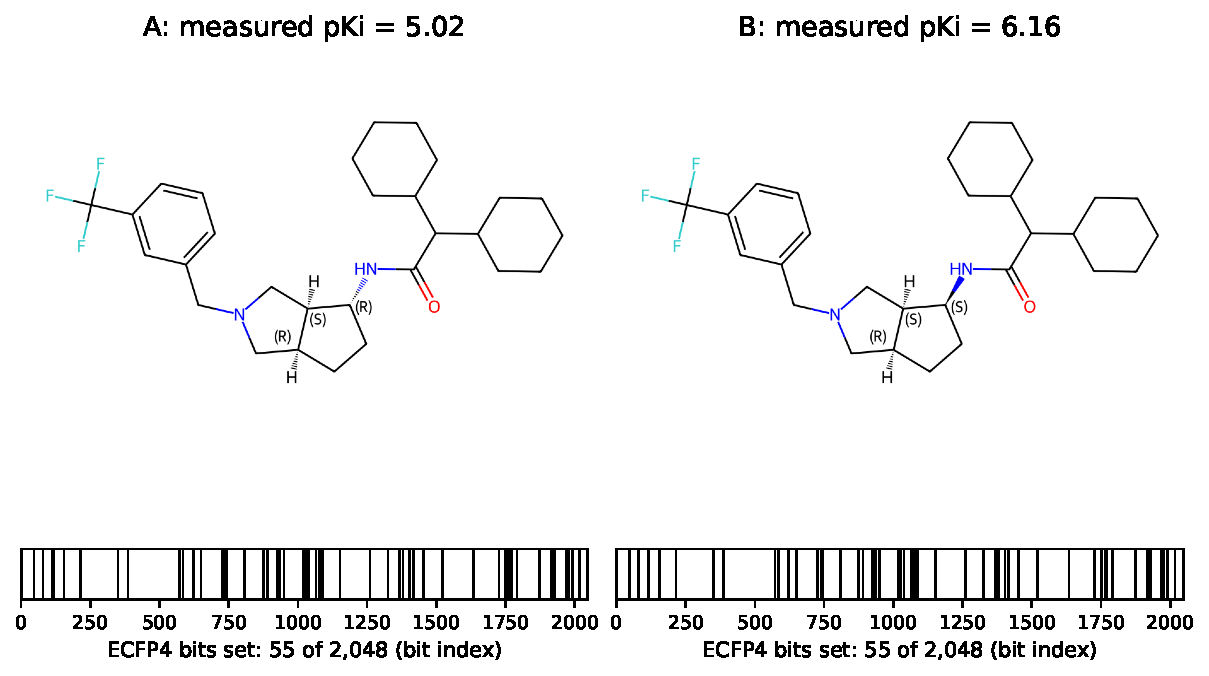
\includegraphics[width=\textwidth,height=0.72\textheight,keepaspectratio]{figures_code_input/herg_ki_ecfp4_stereo_pair.pdf}
\caption[Two hERG $K_i$ stereoisomers with identical ECFP4 vectors.]{Two hERG $K_i$ stereoisomers with identical ECFP4 vectors, which differ at the carbon bearing the amide nitrogen (R in A, S in B). The top row shows the structures with their measured p$K_i$ values, and the bottom row shows the 55 of 2,048 ECFP4 bits set in both.}
\label{fig:flaws:stereo_pair}
\end{figure}

% [TRIM3 2026-09-30] simplified
% Paragraph 6: consequence for activity cliffs and for neighbor-based methods.
The structure--activity landscape index of a pair of molecules $i$ and $j$ is
\begin{equation}
\mathrm{SALI}_{ij} = \frac{|y_i - y_j|}{1 - \mathrm{sim}(i,j)}
\end{equation}
\citep{Guha2008}. A tied pair has similarity 1, so its index is infinite whenever the labels differ. Such a tie is the most extreme activity cliff possible, and an artifact of the representation. A nearest-neighbor method sees a tied neighbor at distance 0 with a different label. % CHECK: sec:flaws:neighbors is not yet a label in thesis.tex; it comes from another CODE INPUT fragment.
It may then flag a correct label as noise (Section~\ref{sec:flaws:neighbors}).

% Table: one row per dataset x representation that ties any molecule.
\begin{table}[htbp]
\centering
\small
\setlength{\tabcolsep}{4pt}
\begin{adjustbox}{max width=\textwidth,max totalheight=0.78\textheight}
\begin{tabular}{llrrrrrr}
\toprule
Dataset & Representation & Molecules & Tied & Stereo- & Best & Best & Largest \\
 & & & & only & RMSE & $R^2$ & spread \\
\midrule
hERG $K_i$ (p$K_i$) & ECFP4 & 1,412 & 56 (4.0\%) & 56 & 0.041 & 0.998 & 1.14 \\
 & Atom pairs & 1,412 & 56 (4.0\%) & 56 & 0.041 & 0.998 & 1.14 \\
 & PDV & 1,412 & 56 (4.0\%) & 56 & 0.041 & 0.998 & 1.14 \\
 & Mordred & 1,412 & 56 (4.0\%) & 56 & 0.041 & 0.998 & 1.14 \\
 & SMI-TED & 1,412 & 56 (4.0\%) & 56 & 0.041 & 0.998 & 1.14 \\
 & Avalon & 1,412 & 66 (4.7\%) & 56 & 0.049 & 0.997 & 1.20 \\
 & WL graph kernel & 1,412 & 105 (7.4\%) & 56 & 0.071 & 0.994 & 1.49 \\
 & MACCS keys (aug.) & 1,412 & 377 (26.7\%) & 30 & 0.134 & 0.978 & 1.80 \\
\midrule
LogD (log units) & ECFP4 & 5,028 & 641 (12.7\%) & 633 & 0.044 & 0.999 & 1.00 \\
 & Mordred & 5,028 & 633 (12.6\%) & 633 & 0.043 & 0.999 & 1.00 \\
 & SMI-TED & 5,028 & 633 (12.6\%) & 633 & 0.043 & 0.999 & 1.00 \\
 & Avalon & 5,028 & 647 (12.9\%) & 629 & 0.047 & 0.998 & 1.40 \\
 & Topological torsions & 5,028 & 675 (13.4\%) & 631 & 0.047 & 0.998 & 1.10 \\
 & MACCS keys (aug.) & 5,028 & 2,343 (46.6\%) & 437 & 0.220 & 0.965 & 2.80 \\
\midrule
Caco-2 (log units) & ECFP4 & 2,158 & 179 (8.3\%) & 177 & 0.027 & 0.996 & 0.74 \\
 & Atom pairs & 2,158 & 177 (8.2\%) & 177 & 0.027 & 0.996 & 0.74 \\
 & PDV & 2,158 & 177 (8.2\%) & 177 & 0.027 & 0.996 & 0.74 \\
 & SMI-TED & 2,158 & 177 (8.2\%) & 177 & 0.027 & 0.996 & 0.74 \\
 & Avalon & 2,158 & 181 (8.4\%) & 177 & 0.027 & 0.996 & 0.74 \\
 & Topological torsions & 2,158 & 186 (8.6\%) & 177 & 0.029 & 0.996 & 0.74 \\
 & WL graph kernel & 2,158 & 203 (9.4\%) & 177 & 0.028 & 0.996 & 0.74 \\
 & MACCS keys (aug.) & 2,158 & 804 (37.3\%) & 139 & 0.111 & 0.935 & 1.72 \\
\bottomrule
\end{tabular}
\end{adjustbox}
\caption[Molecules that share a feature vector with another molecule.]{Molecules that share their feature vector with at least one other molecule, one row per representation that ties any molecules. Tied gives the number and share of such molecules, and Stereo-only those tied only with their own stereoisomers. Best RMSE and best $R^2$ are the best any model can reach given the ties. Best RMSE and Largest spread, the largest label range within one tied group, are in the units beside the dataset name, and (aug.) marks an augmentation representation.}
\label{tab:flaws:ties}
\end{table}

% ==== END CODE INPUT ====




\section{Flaws in Similarity and Other Pairwise Computations}\label{sec:flaws:similarity} % CODE INPUT: label added, needs review
% [notes moved to thesis_notes_moved.md]

% TODO: review, needs manual review
Section~\ref{sec:flaws:representations} described flaws of individual representations. Here we ask what happens when two molecules are compared through one of them. These pairwise comparisons (Chapter~\ref{chap:background}) can violate the similarity assumption, and we discuss both the representation and the coefficient.


The standard way of comparing two small molecules is the Tanimoto coefficient on ECFPs \citep{LopezPerez2024}, although the coefficient applies to any bit vector. Independently, the Tanimoto coefficient is described as the ``coefficient of choice'' for molecular similarity \citep{Bajusz2015}, while the Morgan fingerprint, ECFP4 in this research, ranks among the strongest fingerprints for virtual screening and target prediction \citep{Capecchi2020}. ECFP4 and ECFP6 specifically, alongside topological torsion, rank among the best of 28 fingerprints tested for ordering diverse structures by similarity \citep{OBoyle2016}. However, it is not a one-size-fits-all solution. Across 96,456 human metabolites, 72.9\% had an ECFP4 nearest neighbor at Tanimoto distance 0 \citep{Capecchi2020}, again running into the issue of the representation lacking stereochemical information and more generally being unable to distinguish molecules. 

% [TRIM3 2026-09-30] simplified
% [TRIM 2026-09-30] shortened
% CODE INPUT: references filled in (Equation~\ref{eq:tanimoto_kernel}; the labels sec:flaws:representations, sec:flaws:similarity, sec:flaws:consequences, sec:flaws:constant, sec:flaws:neighbors, sec:lnl_background were added at their headings). Needs review.


All a similarity coefficient can do is compare every feature, yet it cannot tell which features matter to the prediction task at hand. And the similarity assumption holds only relative to such a measure, which is fixed by the choice of representation. To estimate what this costs, we categorize a representation's features into those relevant to the task, $R$, and those that are irrelevant, $I$. We take the squared Euclidean distance as a sum over both:
\begin{equation}
d^2(\mathbf{x},\mathbf{y}) = \sum_{j \in R}(x_j-y_j)^2 + \sum_{j \in I}(x_j-y_j)^2 .
\label{eq:distance_split}
\end{equation}

Every irrelevant feature that varies adds one further term, so the irrelevant part grows linearly with $|I|$. After standardization each feature contributes the same amount on average over all pairs, so the share of the distance carrying signal is about $|R|/(|R|+|I|)$. When we use a general-purpose representation like ECFP4 on a dataset spanning a small portion of the chemical space, $|I|$ can be a lot larger than $|R|$. Features that remain constant across the dataset contribute nothing. Rather, the damage comes from features that vary but bear no relation to the property in question. The worst case scenario involves a single rare bit set in only a handful of molecules. After standardization, uncommon bits take on larger values, outweighing common features that may be more relevant. This is why the near-constant count in Section~\ref{sec:flaws:constant} matters more than the constant count.


Larger representations, or higher dimensionality, compound the problem. As the number of dimensions grows, the nearest and farthest molecules end up at nearly the same distance, meaning that these pairwise distances are less able to discriminate, as explained in Chapter~\ref{chap:background}. Two measures of this effect are the relative contrast, defined as the difference between the largest and smallest measured distance divided by the smallest, and hubness, a measure of how unevenly the molecules appear in other molecules' nearest neighbors \citep{Radovanovic2010}; we do not compute them here. These errors propagate along larger data pipelines, starting from the representation into similarity, from similarity into the set of neighbors a molecule is compared against, and from there into a prediction of some kind. 

% CODE TODO [handled, see CODE INPUT blocks below]: paragraphs 6 + 7 + figure + table, finish this out


% [TRIM3 2026-09-30] simplified
% ==== CODE INPUT: new, needs review ====
% Numbers: /Users/apunt/repos/KIRBy/scratchpad/thesis_code_todo/distance/results_all.json
% Scripts: compute.py, overlap.py, mcs.py, figure.py, collect.py in the same folder.
% Paragraph 5 result (cliff counts) is the first paragraph below; it can move up to Paragraph 5.
% HLM clearance (adme_hlm) is not in Table~\ref{tab:datasets}; drop its rows if it is not a thesis dataset.
% The cliff rule cited to Chapter 2 is so far only in that section's NOTES ("This thesis counts cliffs with a different rule"); its prose must state it.
% [TRIM 2026-09-30] shortened
% [CH3 CHECK 2026-09-30] The rebuilt Chapter 2 does not state a 0.55 rule; it gives the MoleculeACE rule (similarity above 90% under one of three measures, a tenfold difference in K_i or EC50). The opening sentence now says this chapter uses its own rule. Needs your check that this is the intended framing.
% TODO: review, needs manual review
Chapter~\ref{chap:background} defines an activity cliff and gives the MoleculeACE rule, which uses three similarity measures and a tenfold difference in potency. Here we count cliffs with a simpler rule on one measure. A pair is similar at an ECFP4 Tanimoto similarity of at least 0.55, and the activity gap is set per dataset so that 15\% of molecules are cliffs (14.5\% on LogD, as the share moves in steps). The gap therefore varies between datasets (Table~\ref{tab:flaws:distance_summary}). On hERG $K_i$ it is 1.76 p$K_i$, with 211 of the 1,412 molecules cliffs. On QM9, only 1,093 pairs among 9,978 molecules reach 0.55, and the gap is 0.05~eV, or 0.06 times the median absolute deviation of the labels. On the three datasets from the Biogen set (RLM clearance, MDR1--MDCK efflux and HLM clearance) it is 0.20 to 0.34 log units, or 0.50 to 0.60 times the median absolute deviation.

% [TRIM3 2026-09-30] simplified
The count also depends on the representation. Keeping each dataset's gap, we replaced ECFP4 with each other base representation, taking as similar as many of that representation's closest pairs as ECFP4 calls similar. On hERG $K_i$ the number of cliff molecules then ranges from 138 (atom pairs) to 267 (WL graph kernel). Only 57\% to 74\% of the pairs that ECFP4 calls similar are among another representation's closest pairs, and on QM9 1\% to 24\% (Additional file~\ref{app:add:flaws}).

% [TRIM3 2026-09-30] simplified
% [TRIM 2026-09-30] shortened
We ask two questions of a distance. First, across all pairs, does distance track the difference in property? We summarize the neighborhood-behavior plot of \citet{Patterson1996}, descriptor distance against activity difference for every pair, as the Spearman correlation between pair distance and absolute label difference. Second, can each molecule's label be predicted as the mean label of its five nearest neighbors?

% [TRIM3 2026-09-30] simplified
% [TRIM 2026-09-30] shortened
We computed both for every base representation of seven regression datasets: the six small-molecule regression datasets of Table~\ref{tab:dataset_reps} (Chapter~\ref{chap:method}) and HLM clearance, a third Biogen dataset not used elsewhere in this thesis. Binary representations were compared by Tanimoto distance, and all others by Manhattan distance (next subsection) on standardized, non-constant features. For the all-pairs correlation, datasets above 2,000 molecules were reduced to a random sample of 2,000. For the neighbor prediction, each molecule's five neighbors were drawn from other scaffold groups.

% [TRIM3 2026-09-30] simplified
% [RESTORE 2026-09-30] Ch4-7
% TODO: review, needs manual review
Across the 70 combinations of dataset and representation, the all-pairs correlation ranged from $-0.04$ to 0.23 and was below 0.10 in 44 of the 70. The Spearman correlation of the five-neighbor prediction ranged from 0.29 to 0.89, and it was the larger of the two in all 70 (Table~\ref{tab:flaws:distance_summary}). Additional file~\ref{app:add:flaws} gives every representation. On hERG $K_i$, ECFP4 gives an all-pairs correlation of 0.06, while its five-neighbor prediction reaches 0.72, with an RMSE of 0.63 p$K_i$ against a label standard deviation of 0.92 p$K_i$.

% [TRIM3 2026-09-30] simplified
Figure~\ref{fig:flaws:herg_pairs} shows why the two differ on hERG $K_i$. Of the 996,166 pairs, 93\% have an ECFP4 Tanimoto similarity below 0.20 and 1.1\% reach 0.55. The median label difference is 0.81 p$K_i$ over all pairs but 0.20 to 0.30 p$K_i$ above a similarity of about 0.4, though 8.3\% of the 774 pairs at 0.8 or above differ by more than 1 p$K_i$. Under Mordred, the closest 5\% of pairs have a median difference of 0.44 p$K_i$, and every other 5\% a median of 0.78 to 1.11 p$K_i$. The signal sits in this thin tail of close pairs. The all-pairs correlation is set mostly by the other 95\%, whereas a five-neighbor prediction looks only at each molecule's closest pairs.

% [TRIM3 2026-09-30] simplified
% TODO: review, needs manual review
A third view asks how often two representations agree on each molecule's five nearest neighbors, drawn from other scaffold groups. We compared ECFP4, SMI-TED and Mordred (PDV on Caco-2, where Mordred is not a base representation). HLM clearance, which lacks ECFP4 among its base representations, used its stored ECFP4 features. On hERG $K_i$ any two of the three share on average 0.47 to 0.52 of each molecule's five neighbors, and on the three Biogen datasets and QM9 only 0.13 to 0.21 (Table~\ref{tab:flaws:neighbor_overlap}).

% [TRIM3 2026-09-30] simplified
A fourth view asks whether fingerprint distance agrees with a structural distance. For 500 random pairs per dataset we computed the maximum common substructure (MCS) with RDKit \citep{rdkit}, allowing each pair 2 seconds. The MCS distance is $1 - n/(a+b-n)$, where $n$ is the number of atoms in the common substructure and $a$ and $b$ are the numbers of heavy atoms of the two molecules. Its Spearman correlation with ECFP4 Tanimoto distance ranged from 0.20 (hERG $K_i$ and HLM clearance) to 0.51 (Caco-2 and LogD).

% [TRIM3 2026-09-30] simplified
% [RESTORE 2026-09-30] Ch4-9
% TODO: review, needs manual review -- related-work sentences moved to the end of the Introduction's related-work paragraph
Every method in Section~\ref{sec:flaws:consequences} takes a similarity as input and inherits the dilution described here.

\begin{figure}[!htbp]
\centering
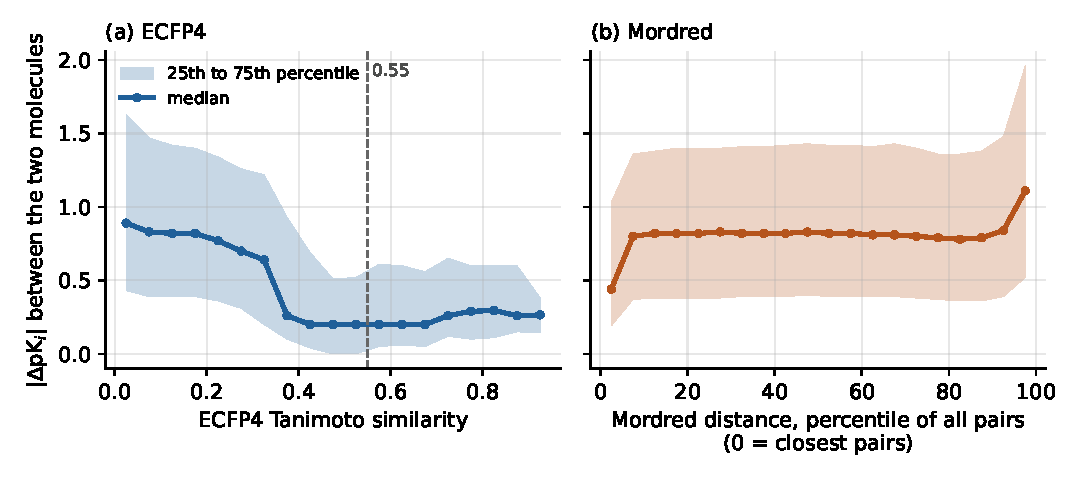
\includegraphics[width=\textwidth,height=0.72\textheight,keepaspectratio]{figures_code_input/herg_ki_pair_distance_vs_dpki.pdf}
\caption[Absolute p$K_i$ difference against pair distance on hERG $K_i$.]{Absolute p$K_i$ difference against distance for all pairs of hERG $K_i$ molecules, with the median in each bin (markers) and the interquartile range (shaded). a) ECFP4 Tanimoto similarity in bins of 0.05 (bins with fewer than 20 pairs omitted), with the activity-cliff threshold of 0.55 dashed. b) Manhattan distance on standardized Mordred features, as a percentile of all pairs.}
\label{fig:flaws:herg_pairs}
\end{figure}


\begin{table}[t]
\centering
\small
\setlength{\tabcolsep}{3.5pt}
\begin{adjustbox}{max width=\textwidth,max totalheight=0.78\textheight}
\begin{tabular}{lrrrrrrrrl}
\toprule
 & & \multicolumn{3}{c}{All pairs} & \multicolumn{3}{c}{Five neighbors} & \multicolumn{2}{c}{Cliffs} \\
\cmidrule(lr){3-5}\cmidrule(lr){6-8}\cmidrule(lr){9-10}
Dataset & Molecules & ECFP4 & Desc. & SMI-TED & ECFP4 & Desc. & SMI-TED & Molecules & Gap \\
\midrule
hERG $K_i$ & 1,412 & 0.06 & 0.07 & 0.09 & 0.72 & 0.72 & 0.69 & 211 & 1.76 p$K_i$ \\
LogD & 5,028 & 0.12 & 0.06 & 0.10 & 0.76 & 0.80 & 0.76 & 731 & 2.90 log \\
Caco-2 & 2,158 & 0.08 & 0.18 & 0.14 & 0.59 & 0.62 & 0.57 & 324 & 1.21 log \\
RLM clearance & 3,053 & 0.02 & 0.07 & 0.04 & 0.36 & 0.49 & 0.46 & 458 & 0.34 log \\
MDR1--MDCK efflux & 2,641 & 0.02 & 0.16 & 0.10 & 0.51 & 0.58 & 0.59 & 397 & 0.20 log \\
HLM clearance & 3,086 & $-0.00$\textsuperscript{\textdagger} & 0.07 & 0.03 & 0.37\textsuperscript{\textdagger} & 0.49 & 0.45 & 462 & 0.27 log \\
QM9 & 9,978 & 0.19 & 0.18 & 0.13 & 0.88 & 0.84 & 0.85 & 1,495 & 0.05 eV \\
\bottomrule
\end{tabular}
\end{adjustbox}
\caption[All-pairs correlation, five-nearest-neighbor prediction and activity cliffs per dataset.]{All-pairs correlation, five-nearest-neighbor prediction and activity cliffs for each dataset. All pairs gives the Spearman correlation between pair distance and absolute label difference, and Five neighbors the Spearman correlation between each label and the mean label of its five nearest neighbors. Cliffs gives the number of cliff molecules and the label gap that defines a cliff. Desc.\ is Mordred, or PDV on Caco-2, and \textsuperscript{\textdagger} marks ECFP4 where it is not a base representation of the dataset.}
\label{tab:flaws:distance_summary}
\end{table}


\begin{table}[t]
\centering
\small
\setlength{\tabcolsep}{4pt}
\begin{adjustbox}{max width=\textwidth,max totalheight=0.78\textheight}
\begin{tabular}{llrrrrrr}
\toprule
 & & \multicolumn{3}{c}{Five-neighbor overlap} & \multicolumn{3}{c}{ECFP4 against MCS} \\
\cmidrule(lr){3-5}\cmidrule(lr){6-8}
Dataset & Desc. & \makecell{ECFP4--\\Desc.} & \makecell{ECFP4--\\SMI-TED} & \makecell{Desc.--\\SMI-TED} & Spearman & Pairs & \makecell{Timed\\out} \\
\midrule
hERG $K_i$ & Mordred & 0.52 & 0.50 & 0.47 & 0.20 & 495 & 5 \\
LogD & Mordred & 0.38 & 0.41 & 0.41 & 0.51 & 494 & 6 \\
Caco-2 & PDV & 0.38 & 0.41 & 0.38 & 0.51 & 492 & 8 \\
RLM clearance & Mordred & 0.15 & 0.21 & 0.18 & 0.28 & 500 & 0 \\
MDR1--MDCK efflux & Mordred & 0.15 & 0.20 & 0.17 & 0.26 & 500 & 0 \\
HLM clearance & Mordred & 0.15 & 0.21 & 0.18 & 0.20 & 500 & 0 \\
QM9 & Mordred & 0.13 & 0.18 & 0.21 & 0.46 & 500 & 0 \\
\bottomrule
\end{tabular}
\end{adjustbox}
\caption[Agreement between representations per dataset.]{Agreement between representations for each dataset. Five-neighbor overlap is the mean fraction of a molecule's five nearest neighbors that two representations share. ECFP4 against MCS gives the Spearman correlation between ECFP4 Tanimoto distance and MCS distance, the number of pairs used, and the number left out because the MCS search timed out.}
\label{tab:flaws:neighbor_overlap}
\end{table}
% ==== END CODE INPUT ====


\subsection{Distance Metrics for Continuous Molecular Descriptors}
% [notes moved to thesis_notes_moved.md]

% [TRIM2 2026-09-30] list cut to the metrics Chapters 5 and 6 use; false pointer to sec:flaws:neighbors dropped
% TODO: review, needs manual review
Binary fingerprints are compared with the Tanimoto coefficient (Chapter~\ref{chap:background}), but continuous features need a distance. The exploratory study of Section~\ref{sec:lnl_motivation} used the following four:

% [TRIM2 2026-09-30] Chebyshev, correlation, Canberra and Bray--Curtis removed
\begin{itemize}
    \item Euclidean ($L_2$): standard geometric distance, $d(x, y) = \sqrt{\sum_i (x_i - y_i)^2}$
    \item Manhattan ($L_1$): sum of absolute differences, $d(x, y) = \sum_i |x_i - y_i|$, more robust to outlier features
    \item Cosine: angle-based, $d(x, y) = 1 - \frac{x \cdot y}{\|x\| \|y\|}$, invariant to magnitude
    \item Mahalanobis: covariance-adjusted distance, $d(x,y)=\sqrt{(x-y)^\top S^{-1}(x-y)}$, where $S$ is the feature covariance estimated on the training molecules \citep{Mahalanobis1936}
\end{itemize}

% [TRIM2 2026-09-30] Bray--Curtis/Canberra sentence removed
All features are standardized to zero mean and unit variance before distances are computed, so that features on different scales contribute equally. % TODO: REVIEW MODIFICATION -- formula checked against the code on 2026-09-29: tests/noise_mitigation_advanced.py:208-219 shifts Bray--Curtis only; Canberra only adds 1e-10. The Mahalanobis covariance matrix is singular here, as the features outnumber the molecules, so its pseudo-inverse is used.

% [TRIM3 2026-09-30] simplified
% [TRIM2 2026-09-30] "four of these" became "four distances": after the list cut, Minkowski is not in the list and Mahalanobis is
% TODO: review, needs manual review
Chapters~\ref{chap:method} and~\ref{chap:similarity} use four distances: Manhattan by default, Euclidean, cosine, and Minkowski with $p=0.5$, $d(x,y)=\left(\sum_i |x_i-y_i|^{0.5}\right)^{2}$, a dissimilarity rather than a metric because it breaks the triangle inequality. Feature weights from the hybrid are applied after standardization (Chapter~\ref{chap:similarity}).


% CODE INPUT: heading added. The notes block below had no \section, but the chapter introduction refers to it as Section~\ref{sec:flaws:consequences}. Needs review.
\section{Consequences for Similarity-Based Methods}\label{sec:flaws:consequences}
% [notes moved to thesis_notes_moved.md]


% [TRIM2 2026-09-30] last sentence ("When I was exploring LNL methods...") deleted
We have identified flaws in the representations themselves and in the similarities computed over them. For a given molecule, its set of neighbors, built from one representation and one distance, is the input to several other processes such as predicting a molecule's activity from its nearest neighbors, detecting noisy labels by comparing a label against its neighbors' labels, defining an applicability domain by distance to the training set \citep{Tropsha2010}, grouping molecules into clusters for data splits \citep{Butina1999}, identifying activity cliffs, and, in federated learning, weighting each site's vote on a molecule by that molecule's distance to the site's own data \citep{Hanser2025}. If the distance is flawed, then every application of distance will suffer the consequences.

Section~\ref{sec:lnl_motivation} reports the exploratory LNL study, in which the 20 configurations with the lowest retention under noise all used a distance. Section~\ref{sec:flaws:neighbors} turns to noise detection by neighbors, the most direct use of similarity in this thesis. 

% CODE TODO [handled, see CODE INPUT blocks below]: so I won't be just reporting my confirmation report. The reviewers won't see that. that material needs to be transferred over, and ideally shortened. this will take a lot... And I have enough there that you can go ahead and copy the langauge (maybe remove some) but refrain from adding your own flair unless it's absoltuely necessary. I've been ignoring every other instruction of yours to cite the confirmation report but now it's unavoidable. This needs fixing. And the output shouldn't be bullets it should just be a smaller version of what I wrote before with results. This should affect this section and the next.
\subsection{Exploratory Study of Learning with Noisy Labels}\label{sec:lnl_motivation}
% [notes moved to thesis_notes_moved.md]

% [OLD TEXT replaced by CODE INPUT below]
% Numerous studies have explored Learning with Noisy Labels (LNL) in the broader context of ML, as well as specifically for QSAR models. \citet{Song2022} provide a comprehensive review of Deep LNL, identifying five main approaches: (i) modifying architectures to better handle noise in training; (ii) employing regularization to reduce overfitting to noise; (iii) adjusting loss functions to be less sensitive to outliers or label flips; (iv) post-processing to adjust the weights for noisy data; and (v) sample selection to select presumably clean data to pre-train. \citet{Cortes2015} examined 12 different algorithms across 12 datasets and 10 noise levels, finding that no single algorithm was overall best at maintaining predictive performance in the presence of noise; certain algorithms perform better or worse at different levels of noise. This is a recurring theme in LNL research: there is no universal solution to handling noise with experimental endpoints.
% % TODO make this flow
% There are a wide variety of approaches to LNL, spanning sample selection, meta-learning, curriculum learning, and iterative refinement \citep{Song2022}. Cheminformatics data presents additional challenges in the form of high-dimensional molecular representations and dealing with a wide variety of chemical domains with various similarities and relationships. In this chapter, we explore a set of 12 LNL methods in the context of QSAR modeling. We examine the impact of uncertainty quantification, molecular distance metrics, and alternative loss functions in the hopes of improving performance under label noise. We tested 221 total configurations across LNL methods, loss functions, distance metrics, and molecular representations. Notably, we found that molecular representation choice explains even less variance under LNL methods. We also identified the following LNL techniques which showed promise on the tasks at hand: heteroscedastic GP, curriculum learning, and sample selection methods. The work was meant to connect the representation and uncertainty quantification insights found in Chapter~\ref{chap:robustness} with more classical noise mitigation techniques as a means of determining broader research directions. 
%
% One of the most prominent outcomes was that distance-augmented methods performed significantly worse than ones that did not incorporate any sense of distance or molecular similarity. An ANOVA test was run on the different adapted factors and shows that distance metric usage is the dominant factor in variance in $R^2$.. When ranking the performance of methods, all 20 worst-performing configurations with respect to noise robustness used distance metrics, not a single one achieved both high baseline ($R^2 > 0.6$) and high noise retention ($> 80\%$). This pattern was observed across standard distance types (Euclidean, Manhattan, Cosine, Mahalanobis) and a chemistry-aware metric (Tanimoto coefficient). 
%
% Building upon the exploratory study above, we decided to investigate alternative featurization techniques. There are multiple possible explanations behind the poor performance of distance metrics, first being that a singular molecular representation lacks sufficient information for distance calculations, with and possibly even without noise. These representations all encode different types of molecular information, PDVs encode global molecular properties, ECFPs contain substructure information, and MPNNs such as MHG-GNNs capture 3D structural features. These single sources of data may not be sufficient for robust similarity estimation. Additionally, some of these representations are sparse and contain a large number of features that are not relevant to molecules of a given domain. 
%
% The main issue we identified here is that when a large proportion of dimensions are uninformative, similarity measures become dominated by those uninformative features, causing exponential growth in the number of irrelevant pairwise interactions as dimensionality increases. This is what we sought to address by developing a representation with informative features and low dimensionality. We do so by creating a budget-constrained hybrid representation, which takes high-importance features from a variety of sources. These hybrid representations concatenate the top-ranked features by importance from a selection of base representations. 
% ==== CODE INPUT: new, needs review ====
% Transferred from the confirmation report (paper.tex, Chapter 4 "Exploring techniques for learning with noisy labels for QSAR", and the opening of Chapter 5), shortened, with the "Change:" bullets applied.
% [TRIM3 2026-09-30] simplified
% TODO: Ch3 update -- re-check the Chapter 3 results quoted in this paragraph against the updated chapter.
% [CH3 CHECK 2026-09-30] re-checked against the rebuilt Chapter 3 Conclusions: model family is the dominant factor for robustness (AUC_norm); representation explains at most 11.2% of its variance.
% [TRIM2 2026-09-30] clean-performance half of the Chapter 3 sentence cut
% TODO: review, needs manual review
This section reuses an exploratory study of LNL carried out earlier in this project. In Chapter~\ref{chap:robustness}, model family explained the largest share of the variance in robustness to label noise, and representation at most 11.2\%, so we asked whether training methods built for noisy labels improve robustness, and whether the representation still matters under them.

% [TRIM3 2026-09-30] simplified
% [TRIM 2026-09-30] shortened
% [RESTORE 2026-09-30] Ch4-10
LNL methods and the five groups of \citet{Song2022} are described in Section~\ref{sec:lnl_background}, and such methods have been studied across machine learning, including QSAR. In the study of \citet{Cortes2015}, gradient boosting tolerated noise worst, SVM and GP models with polynomial kernels were sensitive at high noise in some cases, and the other algorithms degraded smoothly and linearly with the noise level. Most LNL methods were built for image classification with flipped labels \citep{Song2022}, so they do not transfer automatically to continuous labels.

% [TRIM3 2026-09-30] simplified
% [TRIM 2026-09-30] shortened
% [CH3 CHECK 2026-09-30] Sort & Slice citation changed from Dablander2024 (a PhD thesis) to sns, the key Chapters 2 and 3 use.
% TODO: the exploratory study's sigma is not stated to be in the units of the Chapter 2 noise level (a fraction of the clean training-label standard deviation, Equation eq:dose_matching). Check the confirmation-report code; if it is, say so here with a pointer to Section sec:noise_injection.
% TODO: review, needs manual review
The study tested 12 LNL methods on the QM9 HOMO--LUMO gap (10,000 molecules, scaffold splits), adding Gaussian noise with $\sigma$ from 0 to 1.0 in steps of 0.1 to the training labels only. The representations were ECFP4, Sort \& Slice \citep{sns}, PDV, canonical SMILES and randomized SMILES. Depending on the method, a configuration could add the model's own uncertainty, a distance between molecules (Tanimoto, Euclidean, Manhattan, cosine or Mahalanobis), an alternative GP kernel or an alternative loss function, giving 221 configurations. Four methods, small-loss selection, confident learning, distance-based selection and multistage cleaning, remove suspected molecules and retrain. These are noise mitigation methods; the other eight are noise-robust training methods.

% [FIX 2026-09-30] restored 'Methods that used a distance did worse...' (cut by TRIM3) and added the ANOVA finding, both from the exploratory study (Confirmation_Report/paper.tex, LNL chapter, Results); removed 'The same methods without the distance did not fail in this way', which the study does not state.
% TODO: the study says 'all 20 worst-performing configurations ... used distance metrics, not a single one achieved both high baseline (R^2 > 0.6) and high noise retention (> 80%)'. It is ambiguous whether 'not a single one' means the 20 worst or every configuration with a distance. This sentence reads it as every configuration with a distance.
% [TRIM3 2026-09-30] simplified
% TODO: review, needs manual review
We measured noise robustness by retention, $R^2$ under noise divided by $R^2$ with clean labels, as a percentage, which is the retention ratio of Chapter~\ref{chap:robustness} (``Evaluation''). Methods that used a distance did worse than those that did not, and in an analysis of variance over the adapted components, whether a distance was used explained the most variance in $R^2$. All 20 configurations with the lowest retention used a distance, and none with a distance reached both a clean $R^2$ above 0.6 and a retention above 80\%.

% [TRIM3 2026-09-30] simplified
% [TRIM 2026-09-30] shortened
The methods that held up estimate noise from the model's own loss or uncertainty. DivideMix \citep{li2020dividemix} retained the most, 86.7\% (standard deviation 0.4\%), followed by small-loss selection \citep{Han2018} at 84.2\% (2.1\%) and the uncertainty curriculum \citep{Bengio2009} at 82.7\% (3.5\%). The heteroscedastic GP \citep{liu2020} retained 79.0\%, averaged over 15 configurations, with $R^2$ of 0.71 on clean labels and 0.56 at $\sigma = 0.6$, where its retention was measured. The exploratory study does not record this noise level for the other methods. Regularization alone retained less, 73.0\% for Mixup and 74.0\% for sharpness-aware minimization. Under these methods, the choice of representation explained even less variance than in Chapter~\ref{chap:robustness}.

% [TRIM3 2026-09-30] simplified
% [RESTORE 2026-09-30] Ch4-12
% TODO: review, needs manual review
The study used one dataset, one property and one noise condition (Gaussian noise on every training label), and Chapter~\ref{chap:similarity} repeats the question on more datasets and under other noise conditions (Section~\ref{sec:noise_injection}). It also added the distance step to methods designed without one, so poor adaptation is an alternative explanation.

% [TRIM3 2026-09-30] simplified
% [TRIM 2026-09-30] shortened
% [RESTORE 2026-09-30] Ch4-13
The distances may have failed for two reasons, which the evidence here does not separate. First, a single representation may lack the information a distance needs, with and possibly even without noise. PDVs encode global molecular properties, ECFP4 contains substructure information and MHG-GNNs encode the molecular graph \citep{kishimoto2023}, and any one of these sources alone may not be sufficient for robust similarity estimation. Second, some representations are sparse, with many features irrelevant to the molecules of a given dataset (Section~\ref{sec:flaws:similarity}). We sought to address the second with the adaptive hybrid representation (Chapter~\ref{chap:method}), which concatenates the top-ranked features by importance from several base representations.
% ==== END CODE INPUT ====


\subsection{Noise Detection by Neighbors}\label{sec:flaws:neighbors} % CODE INPUT: label added, needs review
% [notes moved to thesis_notes_moved.md]

% [OLD TEXT replaced by CODE INPUT below]
% Overall, we see in agreement with conclusions of Section~\ref{sec:lnl_motivation} on the use of distance metrics in LNL methods, the concept of using a sample's neighbors to determine it's ground truth is flawed. It is likely all labels are too uniformly noisy for a methodology like this. Uncertainty-based methods show potential at lower noise, but their estimation performance degrades with higher noise. Sampling weighting methods generally proved effective, and one estimator using exponential sample weighting produced very strong recovery across both noise levels.
%
% Hybrid representations had mixed results. For sample removal, hybrids showed advantages at high noise, but struggled at low noise. They showed consistently positive recovery rates for neighbor-based estimation, which roughly falls in line with the idea that a low-dimension, high-quality information representation benefits neighbor-based reasoning. The feature budget in this experiment was restricted to 50-100 features, which may limit its advantages. This range was successful at standard molecular property prediction, but potentially not for certain noise mitigation or estimation tasks. Distance-based methods remain challenging under Gaussian noise regardless of representation, suggesting the core issue is the noise distribution rather than representation quality alone. This merits an investigation into mitigation of noise from other distributions or noise injection strategies.
% ==== CODE INPUT: new, needs review ====
% Transferred from the confirmation report (paper.tex, Chapter 5 "Noise Estimation" results, lines 1028-1146), shortened, with the "Change:" bullets applied.
% [TRIM3 2026-09-30] simplified
% [TRIM 2026-09-30] shortened
Neighbor-based noise detection treats a label far from its neighbors' labels as probably wrong, an idea that goes back to editing nearest-neighbor training sets \citep{Wilson1972}. The wider literature on filtering noisy labels concerns classification \citep{Brodley1999, frenay2014classification}. \citet{Martin2021} adapt fourteen classification noise filters to regression, seven of them nearest-neighbor filters that use the neighbors' mean label. They find that the filters improve regression methods on 20 general regression benchmarks with injected label noise, none of them QSAR datasets.
% Source needed (from her NOTES, still open): a QSAR source for removing or down-weighting a molecule because its label disagrees with its nearest neighbors' labels.
% [TRIM 2026-09-30] shortened
The neighbor-based noise scores, sample removal, sample weighting, label smoothing and the recovery rate are defined in Chapter~\ref{chap:similarity}, ``Noise mitigation methods''.

% [TRIM3 2026-09-30] simplified
The method needs a distance that picks the right neighbors, and neighbors with clean labels. Earlier sections of this chapter argue that the first condition fails, and the second fails whenever noise is spread over the whole training set. A large gap from the neighbors' labels can mean a noisy label, a noisy neighbor or the wrong neighbors, and the score cannot tell which. Activity cliffs also look like noise to such a detector (Chapter~\ref{chap:background}, ``Molecular similarity and activity cliffs'').

% [TRIM3 2026-09-30] simplified
% [TRIM 2026-09-30] shortened
% [RESTORE 2026-09-30] Ch4-14
The exploratory study also used neighbors to clean labels, on 5,000 randomly chosen QM9 molecules (HOMO--LUMO gap, scaffold split) with Gaussian noise on the training labels at $\sigma = 0.3$ and $\sigma = 0.6$. Each cleaning method was judged by retraining a random forest on ECFP4 with clean, noisy and cleaned labels, giving the recovery rate, the share of the $R^2$ lost to noise that cleaning recovers (Equation~\ref{eq:recovery}). Neighbor-based scores compared each label with those of the molecule's $k$ nearest training molecules under Euclidean, Manhattan or cosine distance. Table~\ref{tab:code_input_neighbor_recovery} holds only the configurations built on a single representation; those built on an early hybrid are described below. This study is separate from the sample-removal study of Chapter~\ref{chap:similarity}.

% [TRIM3 2026-09-30] simplified
With the neighbor-based scores used as sample weights at strength $\alpha = 0.1$, mean recovery was negative for every representation at both noise levels (Table~\ref{tab:code_input_neighbor_recovery}). Of all 860 cleaning configurations, 8 had positive recovery at both noise levels; 6 of these used a single representation, and 4 of those 6 were neighbor-based. Label smoothing toward neighbor or model estimates gave positive recovery in 5.0\% of configurations at $\sigma = 0.3$ and 0.8\% at $\sigma = 0.6$. Mean recovery was negative at every weighting and smoothing strength tried, from 0.1 to 0.7.

\begin{table}[htbp]
\centering
\begin{adjustbox}{max width=\textwidth,max totalheight=0.78\textheight}
\begin{tabular}{lcccc}
\toprule
 & \multicolumn{2}{c}{Mean recovery (\%)} & \multicolumn{2}{c}{Positive (\% of configurations)} \\
\cmidrule(lr){2-3}\cmidrule(lr){4-5}
Representation & $\sigma = 0.3$ & $\sigma = 0.6$ & $\sigma = 0.3$ & $\sigma = 0.6$ \\
\midrule
ECFP4   & $-3.0$ & $-7.3$ & 33.3 & 16.7 \\
PDV     & $-2.4$ & $-3.4$ & 50.0 & 27.8 \\
MHG-GNN & $-0.1$ & $-7.2$ & 38.9 & 5.6 \\
\bottomrule
\end{tabular}
\end{adjustbox}
\caption[Recovery with neighbor-based sample weights by representation.]{Recovery rate in $R^2$ on the QM9 HOMO--LUMO gap when neighbor-based noise scores are used as sample weights, for each representation used to find the neighbors, at two levels $\sigma$ of Gaussian label noise. Recovery is the share of the $R^2$ lost to noise that cleaning regains, so negative values mean cleaning made the model worse. Positive is the share of configurations with recovery above zero.}
\label{tab:code_input_neighbor_recovery}
\end{table}

% [TRIM3 2026-09-30] simplified
Judging a label by its neighbors usually made the model worse and rarely helped at both noise levels, but it did not always fail. The best configuration at $\sigma = 0.6$ was neighbor-based (PDV, Euclidean distance, local variance ratio score) and recovered +17.2\%. Because noise was added to every training label, the neighbors' labels are noisy too; the exploratory study gave this as the reason label smoothing failed.

% [TRIM3 2026-09-30] simplified
% [TRIM 2026-09-30] shortened
Uncertainty-based methods, which use no neighbors, showed potential at lower noise but degraded at higher noise. Sample weighting did better than label smoothing but usually still hurt, with positive recovery in 14.2\% of configurations at $\sigma = 0.3$ and 4.7\% at $\sigma = 0.6$, and mean recoveries of $-22.9\%$ and $-20.9\%$.

% [TRIM3 2026-09-30] simplified
% [TRIM 2026-09-30] shortened
% TODO: review, needs manual review
The study also found neighbors in an early hybrid of 100 PDV and MHG-GNN features, built by greedy forward selection, which is no longer part of the method. Its mean recovery with neighbor-based scores was $-0.9\%$ at $\sigma = 0.3$ and $-3.0\%$ at $\sigma = 0.6$, with 44.4\% and 27.8\% of configurations positive. Chapter~\ref{chap:similarity} repeats the measurement in a hybrid and under noise conditions other than Gaussian.
% ==== END CODE INPUT ====

% CODE TODO [handled, see CODE INPUT blocks below]: give me a sample to finish this out. Keep the relatively plain langauge style I've been working with, but I suspect this will change based on results a bit. Or not. I could just use some paragraphs on it. Don't go crazy, a conclusion is supposed to distill what's been done into something readable, something to remind the reader about the big picture before they walk away. Simple. 
\section{Conclusions}
% [notes moved to thesis_notes_moved.md]
% ==== CODE INPUT: new, needs review ====
% Sample conclusion following NOTES Paragraphs 1-6 and the Table. No new evidence.
% Every number is copied from another CODE INPUT fragment of this chapter:
%   Paragraph 1: out/constant.tex (constant/constant_counts.json) and out/ties.tex (ties/ties_results.json).
%   Paragraph 2: out/distance.tex (distance/results_all.json).
% If those fragments change, these numbers must change with them.
% [TRIM3 2026-09-30] paragraph removed

% [TRIM3 2026-09-30] simplified
% [RESTORE 2026-09-30] Ch4-16
On a single dataset, often very little of a standard representation varies. On hERG $K_i$, 1,815 of the 2,048 ECFP4 features take one value in at least 95\% of the 1,412 molecules (Section~\ref{sec:flaws:constant}). Several representations also give different molecules, mostly stereoisomers, the same feature vector, and no model can separate those molecules, whatever their labels. ECFP4 gives 56 of the 1,412 hERG $K_i$ molecules a vector shared with another molecule, all of them stereoisomers (``Molecules with identical feature vectors'').

% [TRIM3 2026-09-30] simplified
A distance sums over every feature, so when only a few features matter for the property, the rest dominate the sum (Section~\ref{sec:flaws:similarity}). Across 70 combinations of dataset and representation, the Spearman correlation between pair distance and label difference was below 0.10 in 44. % CHECK: NOTES say keep the all-pairs vs nearest-neighbor contrast only if the full runs support it. The numbers below come from distance.tex, computed on the saved features, not from the full runs.
Predicting each label from its five nearest neighbors gave a higher Spearman correlation in all 70, so the useful information sits in a few close pairs rather than in the distance as a whole.

% [TRIM3 2026-09-30] simplified
% [RESTORE 2026-09-30] Ch4-17
% TODO: review, needs manual review
In the exploratory LNL study, configurations that used a distance did worst under label noise (Section~\ref{sec:lnl_motivation}), and judging a label by its neighbors' labels usually made the model worse (Section~\ref{sec:flaws:neighbors}). It did not always fail, since one neighbor-based configuration gave the best recovery at the higher noise level. That noise was Gaussian on every training label, so each molecule's neighbors were noisy too; Chapter~\ref{chap:similarity} turns to the other noise conditions of Chapter~\ref{chap:background}.

% [TRIM3 2026-09-30] simplified
A representation that avoids these flaws would need five properties (Table~\ref{tab:flaws:requirements}). Its features would be chosen for the task, using only each fold's training labels. It would be compact, dropping features that do not vary or do not matter, with the number kept searched rather than fixed. It would draw on several representations, since each misses information the others capture; plain concatenation does this but is not compact (Chapter~\ref{chap:method}, ``Combining representations and the alternatives''). It would work both as a model input and as a space for similarity. Finally, it would be traceable: each chosen feature leads back to its representation and can be read chemically wherever the base feature can.

% [TRIM3 2026-09-30] simplified
Feature selection cannot fix every flaw. Molecules identical in every base representation stay identical in the hybrid, and a selected hashed bit still merges every substructure folded into it. Selection also needs enough labeled molecules to estimate which features matter.

% [TRIM2 2026-09-30] cut to one bridging sentence with a back-reference to Chapter 1
% [TRIM4 2026-09-30] c4_flaws-P6: added one sentence pointing to Chapter 5's ``The Search Space'' in place of the settings list TRIM3 removed
% TODO: review, needs manual review
These flaws are where the thesis began (Chapter~\ref{chap:intro}), and Chapter~\ref{chap:method} builds the method they led to, the adaptive hybrid representation. The settings that method searches over are listed in Chapter~\ref{chap:method}, ``The Search Space''.

% [TRIM3 2026-09-30] paragraph removed

% [TRIM3 2026-09-30] paragraph removed

\begin{table}[htbp]
\centering
\small
\begin{adjustbox}{max width=\textwidth,max totalheight=0.78\textheight}
\begin{tabular}{P{0.34\textwidth}P{0.30\textwidth}P{0.28\textwidth}}
\toprule
Flaw (where shown) & Requirement & Where handled \\
\midrule
Features that do not vary (``Constant and near-constant features'') & Features chosen for the task, within a budget & ``Feature importance scoring'' \\
Molecules merged into one vector (``Molecules with identical feature vectors'') & Features drawn from several representations & ``Combining representations and the alternatives'' \\
Distance dominated by irrelevant features (``Flaws in similarity and other pairwise computations'') & Compact, with the number of features searched & ``The search space'' \\
Poor performance of neighbor-based methods (``Consequences for similarity-based methods'') & Usable as a space for similarity & ``Similarity in a hybrid'' (Chapter~\ref{chap:similarity}) \\
% [TRIM2 2026-09-30] fifth row (traceable) added to match the five properties in the prose
% TODO: review, needs manual review
Features that are hard to read chemically (``Flaws in standard base representations'') & Traceable, so that each chosen feature leads back to its representation and can be read chemically wherever the base feature can & ``Blueprints and their chemical interpretation'' \\
\bottomrule
\end{tabular}
\end{adjustbox}
\caption[Flaws of standard representations and similarity, and the requirement each sets.]{Flaws of standard representations and similarity, the requirement each sets for a representation, and where the requirement is addressed, in Chapter~\ref{chap:method} unless stated.}
\label{tab:flaws:requirements}
\end{table}
% ==== END CODE INPUT ====


 % Context for similarity and my motivating hypothesis: I think that molecular similarity as we often do it (ECFP4/Tanimoto or other variations of that) is flawed and applications that this concept of similarity (in my case noise detection and mitigation) suffer as a result
 %    - Take a look at ECFP4 as an example. Let's say you're working with molecules in a particular domain, how many of those features are going to useless? First, you can get numbers on in a given dataset how many features have no difference between the molecules. Some will differ, but will have nothing to do with the task at hand. There's definitely useful features in that set of 2048, but they're probably quite sparse, and when you take a similarity metrix that does a vector by vector comparison, and some of your features are irrelevant, you have exponentially more irrelevant pieces of information (is this true? phrase this better). I thought a much more efficient approach would be to select useful features for that task (I define task as some kind of supervised model fit on a training set) and you specify how many features you want, and you use that to calculate similarity. Now I implemented a proof-of-concept version of this and realized that these customized feature sets (hybrids) work as standard inputs to the model, irregardless of similarity. Then the main question was how on earth do I select the best features? How do I score how meaningful a feature is (feature importance), if I have lots of base reps, how do I know how many features from each to select (allocation strategies), once I have a candidate, how do I score it to see if its useful (internal evaluator). Then the other axes I test for the purposes of seeing if this works: does it work on different downstream evaluators, and what happens when I modify/control the budget (number of features).
 %        - Compare to other feature selection algorithms but explain why this is different - you could just pool all the features (and I've tried this, pull up my results on it), but it's not actually as effective as looking at them on a representation-level. It turns out if you have 10 reps you're considering, and you limit it to the top 2,3, 5, SOME datasets prefer that. Others prefer all 10. It's more complex than a simple feature selection algorithm if you really want to optimize it, and my results show why
 %        - This use case is specifically taking existing reps that say vastly different things about the molecule (PDV vs ECFP4 vs graph based embeddings vs sequence based embeddings) and tailor selecting a set of features from all of these to the very specific task at hand
 %    - Two concepts of using similarity: make a normal hybrid and use it for similarity OR modify the objective that the hybrid search optimizes for to make it similarity-aligned (called "similarity hybrids")
